\section{Iteration 5: Decomposition of the Scheduler for Anomaly Detection}
\label{add:it5}

\subsection{Step 1: Identify candidate drivers}
\label{add:it5/drivers}

\npar This iteration is driven by:

\begin{itemize}
	\item P1': Timely closure of valves. Alarm trames have to be handled within a bounded time. 
	\item P2': Anomaly Detection. When the system is in overload modus the processing order of trames
	  occurs on a priority basis (premium service has a higher priority than
	  normal service).
\end{itemize}

\npar No use cases were delegated to this component.

\subsection{Step 2: Choose design concepts}
\label{add:it5/concepts}

\npar The design concepts for this decomposition are completely analogous to the
design concepts of iteration 3 (see section \ref{add:it3/concepts}), since it
involves scheduling as well.

\subsection{Step 3: Instantiate architectural elements and allocate responsibilities}
\label{add:it5/elements}

\npar Also analogous to iteration 3 (see \ref{add:it3}), an ADScheduler will
enqueue processing jobs with a priority in an ADQueue with an ADPolicy. An
ADQueueReader will dequeue jobs from the queue and feed them
to the Anomaly Detection Unit. 

\npar An overview of the instantiated child components of the Scheduler
For Anomaly Detection is shown in \ref{fig:it5/elements}.

\subsubsection{ADScheduler}

\npar This scheduler regulates all the traffic of ADCommands towards the
Anomaly Detection Unit. It accepts incoming ADCommands at a random rate (i.e.
the rate at which the communication and storage send them towards this
component) and it redirects them to the Anomaly Detection Unit. This
scheduler guarantees in addition that the rate at which it will send the
ADCommands to the Anomaly Detection Unit will not exceed its maximum sending
rate.

\subsubsection{ADPolicy}

\npar An ADPolicy is responsible for inserting incoming ADCommands (received
from the ADScheduler) into the ADQueue. To be able to do this, the policy first
has to determine the priority of the incoming command (and this priority is
different for the various policies).

\subsubsection{ADQueue}

\npar The ADQueue does nothing else than provide a priority queue for
ADCommands with accompanying insert and retrieve functionality. Since
it is a priority queue, the commands can be placed in different places in the
queue depending on their priority. More precisely, for each priority level will
the index of the last element with that priority be kept in a list. When a new
command needs to be inserted, the priority of that command is determined.
Subsequently, the priority is used to retrieve the index of the last element and
in this way the new command can be inserted.

\subsubsection{ADQueueReader}

\npar The purpose of this component is dequeueing the ADQueue and
afterwards dispatch the popped command to the the Anomaly Detection Unit.

\begin{figure}[H]
	\begin{centering}
		% TODO Figure
		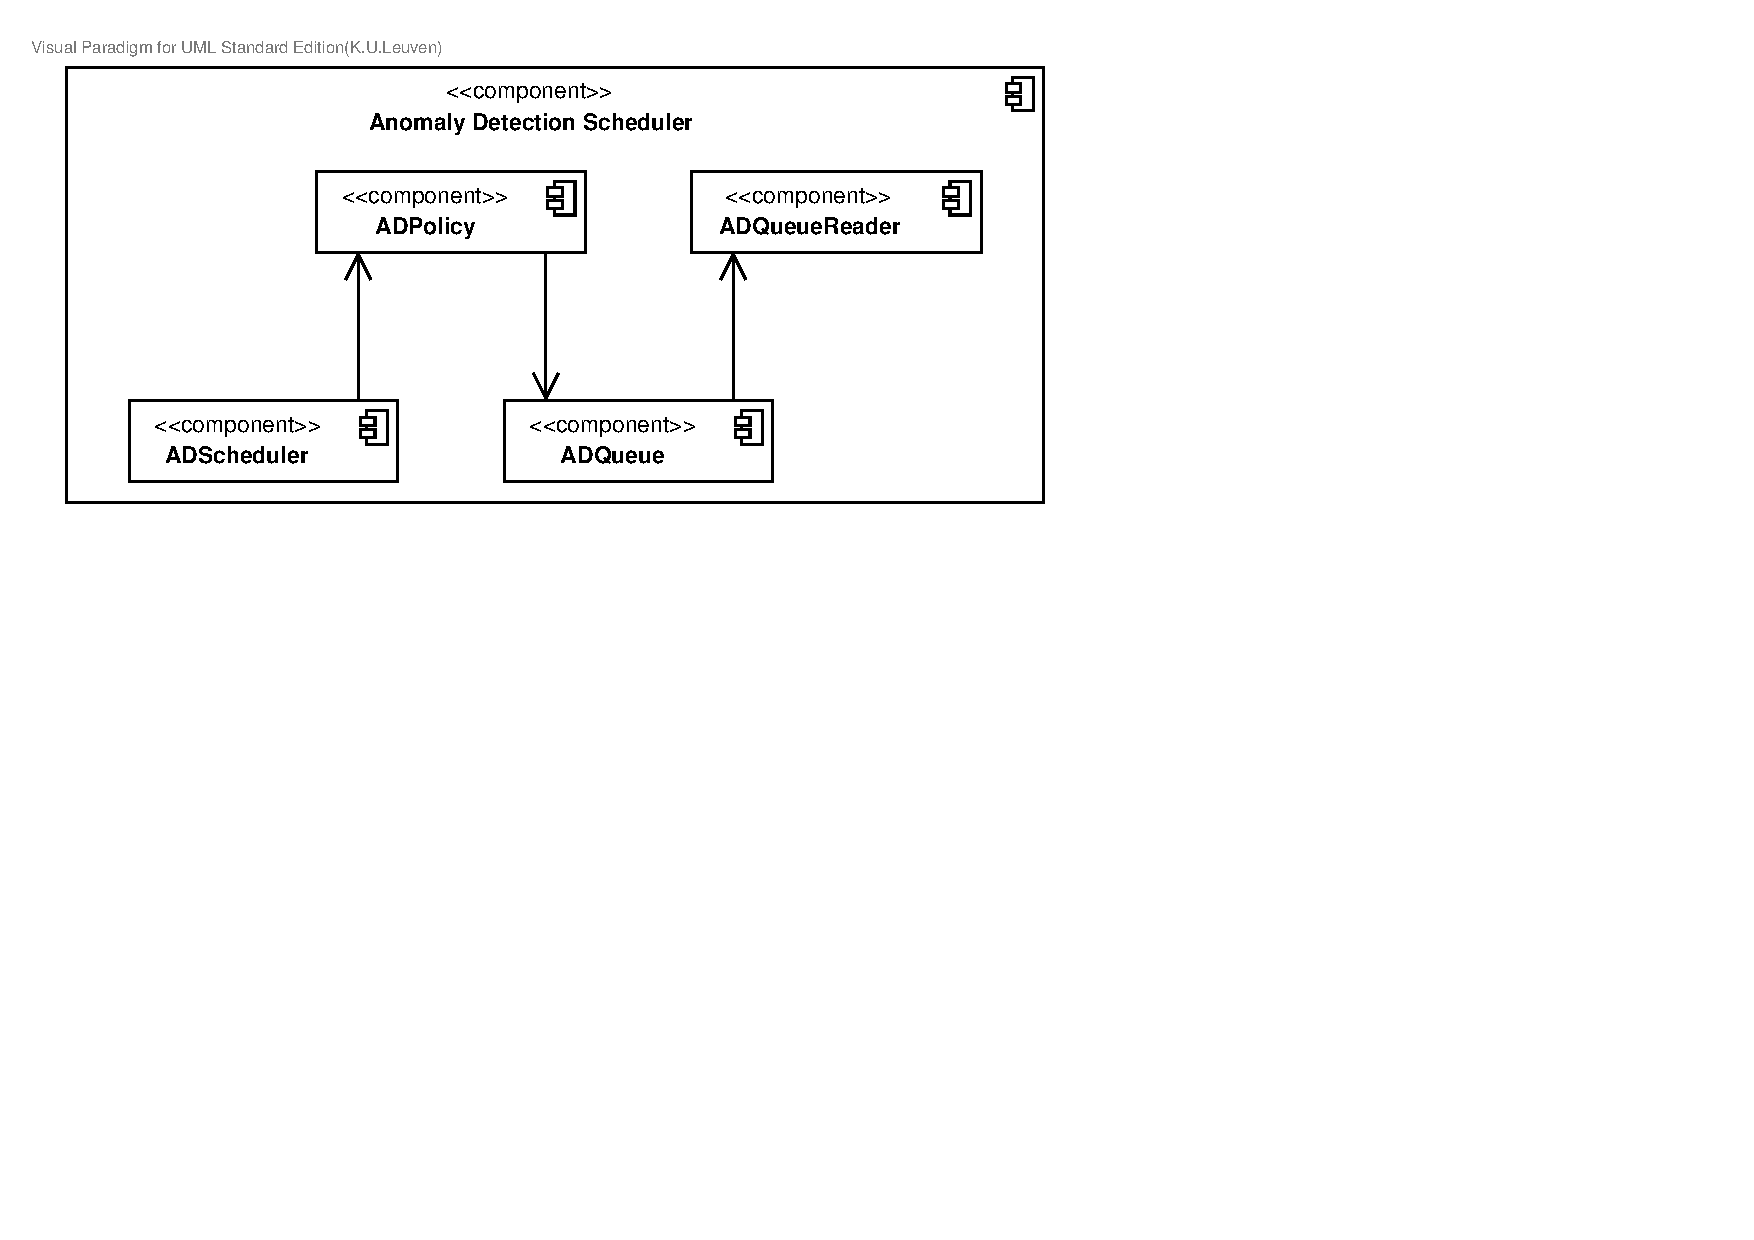
\includegraphics[width=\textwidth]{figs/add-it5-elements.pdf}
		\caption{Overview of all instantiated child elements in the Anomaly
		Detection Scheduler}
		\label{fig:it5/elements}
	\end{centering}
\end{figure}

\subsection{Step 4: Define interfaces for instantiated elements}
\label{add:it5/interfaces}

\npar In this section each interface is explained in terms of the components
which use and/or offer it together with information about what is exchanged. For
detailed information with reference to the specific methods the interfaces
implement, we refer to the interface catalog, see appendix
\ref{chap:interface-catalog}.

\npar Because this scheduler is very similar to the measurements scheduler from
iteration 3 (see \ref{add:it3}), the interfaces are also very similar.

\subsubsection{ADSchedulerAPI}

\npar This interface was already discussed in iteration 1, see
\ref{add:it1/interfaces}.

\subsubsection{ADPolicyAPI}

\npar The \interface{ADPolicyAPI} lies between the ADScheduler and the ADPolicy.
Its goal is to pass through commands which have to be placed in an ADQueue.

\subsubsection{ADQueueAPI}

\npar This interface is offered by the ADQueue and used by both the ADPolicy and
the ADQueueReader. The policy uses the interface to place commands in the queue
and the reader pops them off.

\npar Figure \ref{fig:it5/interfaces} summarizes the components and the
interfaces instantiated in this iteration.

\begin{figure}[H]
	\begin{centering}
		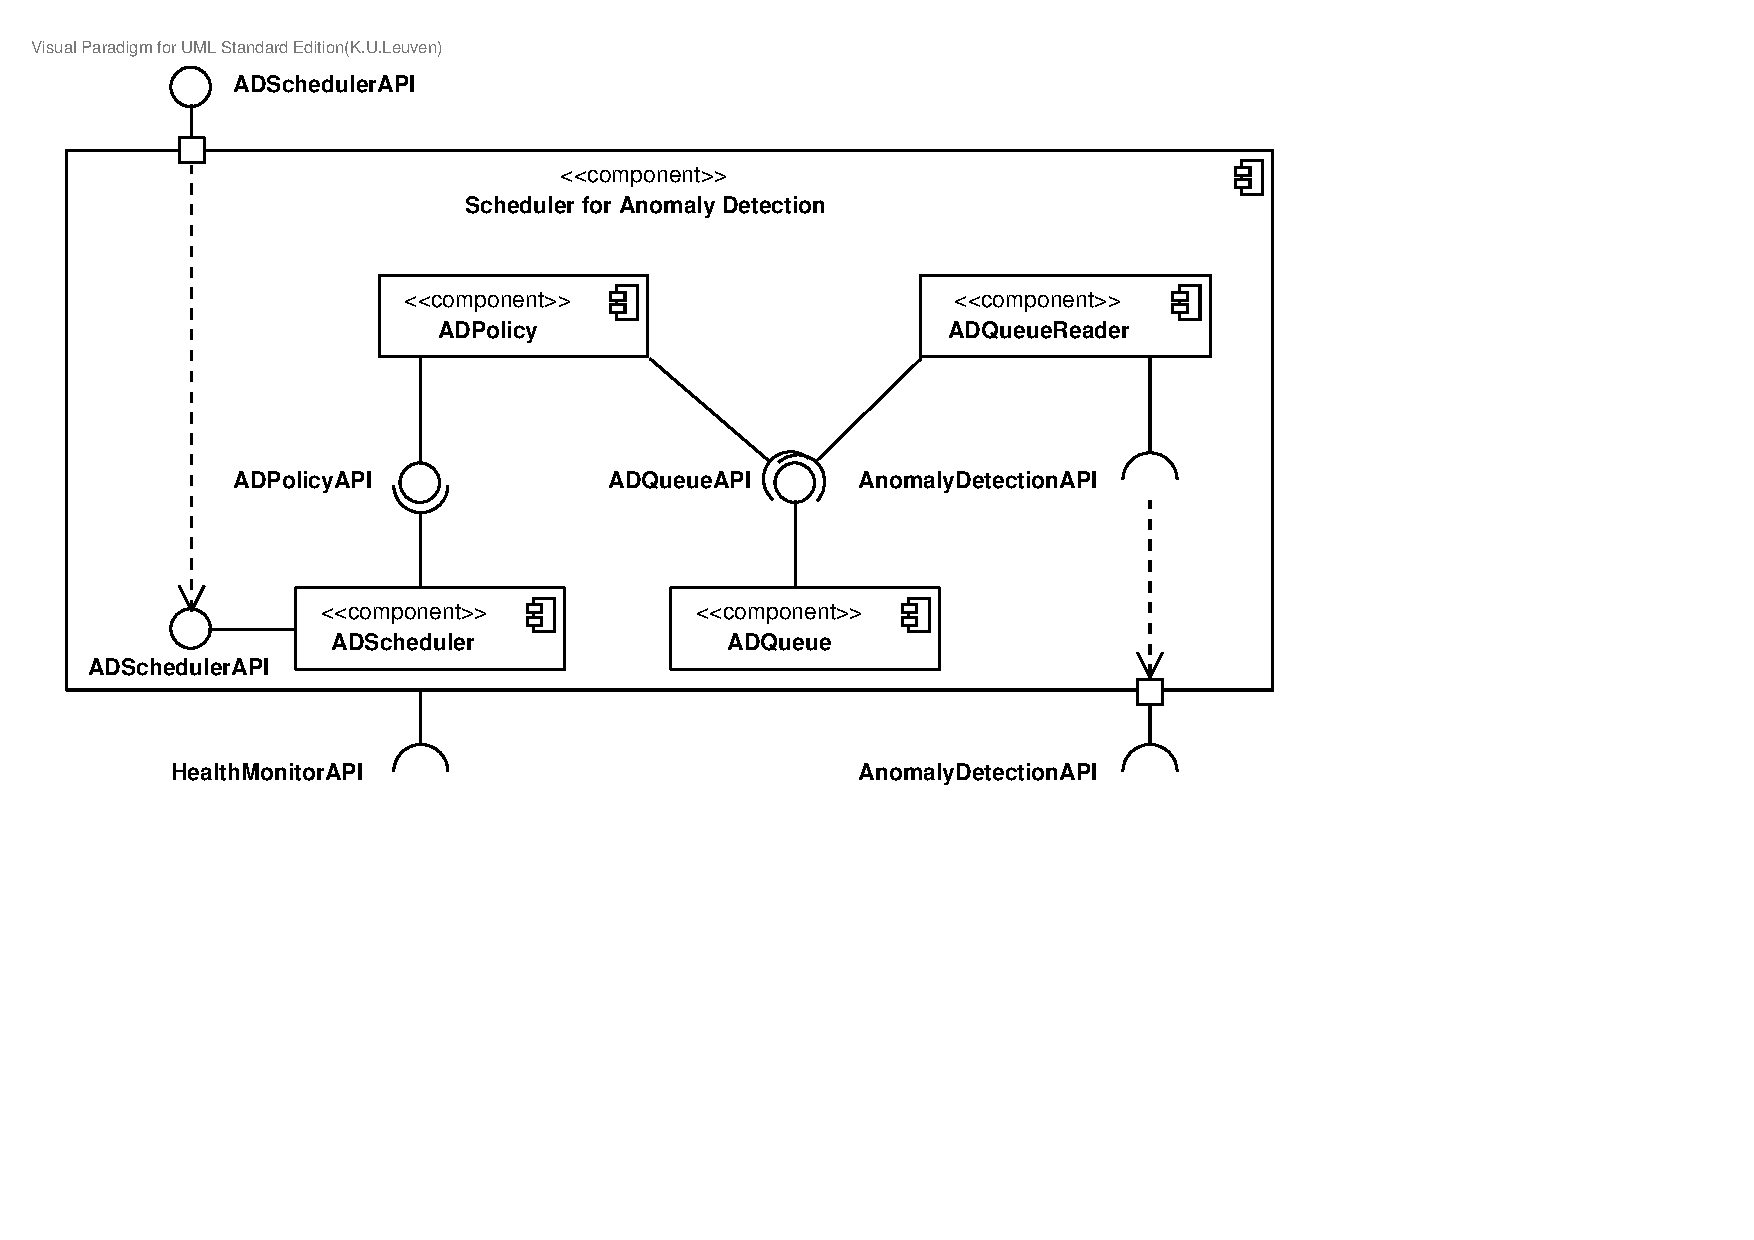
\includegraphics[width=\textwidth]{figs/add-it5-interfaces.pdf}
		\caption{Overview of the interfaces and components in the Scheduler For
		Anomaly Detection.}
		\label{fig:it5/interfaces}
	\end{centering}
\end{figure}

\subsection{Step 5: Verify and refine}
\label{add:it5/verification}

\npar All quality requirements are resolved in this iteration. The policies for
the scheduler will ensure that commands are scheduled in the right order. 
